\chapter{Desenvolvimento}
Esta documentação está dividida em duas partes principais. A primeira delas, Seção \ref{sec:papel}, apresentará qual é o papel do Portal \ppod, como ele irá se relacionar com as demais iniciativas. A segunda delas, Seção \ref{sec:recursos}, vai apresentar as principais modificações que foram implementadas ou que deverão ser implementadas no projeto \ppod.

\section{Papel}\label{sec:papel}
O portal \ppod foi criado para promover a democratização do processo de elaboração legislativa no Brasil.

A principal ação promovida no âmbito do projeto é a mobilização de setores importantes da sociedade – Academia, instituições de pesquisa, ONG’s entre outros – para a realização de estudos em temas de interesse da Secretaria.
	
Porém, as ações da \gls{sal} no sentido de democratizar o processo de elaboração legislativa se expandiu para contemplar também consultas públicas para legislações em produção.

Até o início da presente consultoria, tais consultas não eram realizadas como parte do projeto \ppod, mas sim como partes de um ``meta-projeto'' chamado ``Participação'', atuando ``em paralelo'' ao \ppod.

Após diversas reflexões da equipe, decidiu-se que a melhor opção seria remodelar este fluxo utilizando o Portal \ppod como um ``guarda-chuva'' de diversas iniciativas, dentre elas as consultas públicas.

Dessa forma, o Portal \ppod passa a ser o portal das iniciativas de participação social da \gls{sal}, sendo elas:

\begin{description}
\item[Publicações] Estudos realizados em parceria com acadêmicos e especialistas;
\item[Debates] Consultas e Debates Públicos realizados por meio de plataformas específicas;
\item[Proponha um Debate] Ferramenta para que a população proponha um \textbf{Debate} a ser realizado;
\item[Programa de Intercâmbio] Blog para divulgação das atividades do Programa promovido pela \gls{sal};
\item[Agenda] Agenda oficial da \gls{sal} e do Secretário; e
\item[outras] que venham a surgir.
\end{description}

\section{Implementação de Recursos e Principais Diretrizes}\label{sec:recursos}
\subsection{Endereços}
Um ponto importante de ser definido é a padronização de endereços (urls) relativos ao projeto \ppod e todas as iniciativas que derivam dele.

Atualmente o endereço principal utilizado é o \url{http://participacao.mj.gov.br}. Com a finalidade de fortalecer a marca \ppod, e remover uma confusão entre o ``\ppod'' e o ``Portal de Participação Social do Ministério da Justiça'' - que deixa de existir e passa a ser o próprio portal do ``Pensando''; o endereço atual deverá ser redirecionado para o novo endereço a ser utilizado \url{http://pensando.mj.gov.br}, que passa a ser o endereço oficial do projeto e que deve ser utilizado nas divulgações a partir do momento da efetivação da mudança.

Outro ponto diz respeito ao endereço das consultas públicas. Cada uma das consultas públicas realizadas possuia um endereço (subdomínio) próprio (ex.: \url{http://marcocivil.mj.gov.br}). A vantagem deste modelo é que ele destaca a consulta que está sendo realizada, e permite que se defina um endereço consideravelmente curto e fácil de memorizar/divulgar.

Porém, este modelo apresenta duas principais desvatagens. A primeira delas é que ele dificulta encontrar quais são as consultas em vigor, ou realizadas, visto que não há um padrão de endereço para as consultas públicas.

Outra desvantagem é que este modelo acaba por desfavorecer a marca do \ppod, em especial no que diz respeito ao endereço, e prejudica também o desempenho do endereço em sistemas de busca e de redes sociais, já que o endereço principal do pensando acaba tendo seu público dividido e segmentado com outros endereços (das consultas).

Assim, acordou-se que os endereços das próximas consultas (debates) públicas estarão ficarão sob o endereço do projeto \ppod, preferencialmente como: \textit{http://pensando.mj.gov.br/debate/<nome\_do\_debate>}, padronizando assim o endereço de todas as consultas e debates e também reforçando o endereço do projeto.

Após a implementação deste modelo de endereços, três ações são importantes de serem realizadas.

A primeira ação é revistar os conteúdos publicados no portal, realizando a substituição dos endereços antigos pelos novos formatos. Esta tarefa pode ser realizada por meio de busca e substituição tanto nos códigos-fonte do projeto quanto nas bases de dados do projeto.

A segunda ação é a mudança dos endereços nos perfis de redes sociais (Twitter, Facebook, Instagram) utilizados (Pensando O Direito, Marco Civil da Internet, Dados Pessoais, etc).

A terceira ação é a configuração dos servidores para que eles redirecionem os endereços antigos para os novos endereços, evitando que algum usuário que tenha acesso aos endereços antigos não consiga acessar o conteúdo ou acesse um conteúdo desatualizado.

\subsection{Publicações}
Para as \textbf{Publicações} da série \ppod foi criado um \gls{cpt} do Wordpress, chamado ``\textit{publicacao\_post\_type}'', e as diversas páginas necessárias (\textit{archive-publicacao.php}, \textit{content-publicacao.php}, \textit{publicacao-card.php}, \textit{sidebar-publicacao.php} e \textit{single-publicacao.php}). O \gls{cpt} criado pode ser observado no arquivo \textit{functions.php} do projeto \textit{pensandoodireito-tema}\footnote{Arquivo \textit{functions.php} do projeto \textit{pensandoodireito-tema} no github: \url{https://github.com/pensandoodireito/pensandoodireito-tema/blob/master/functions.php}}.

\subsubsection*{Página Principal}
Para as \textbf{Publicações} da série \ppod foi desenvolvida uma área dedicada, conforme pode ser observado na Figura \ref{fig:publicacoes-geral}.

\begin{figure}[Htb]%
	\begin{center}
		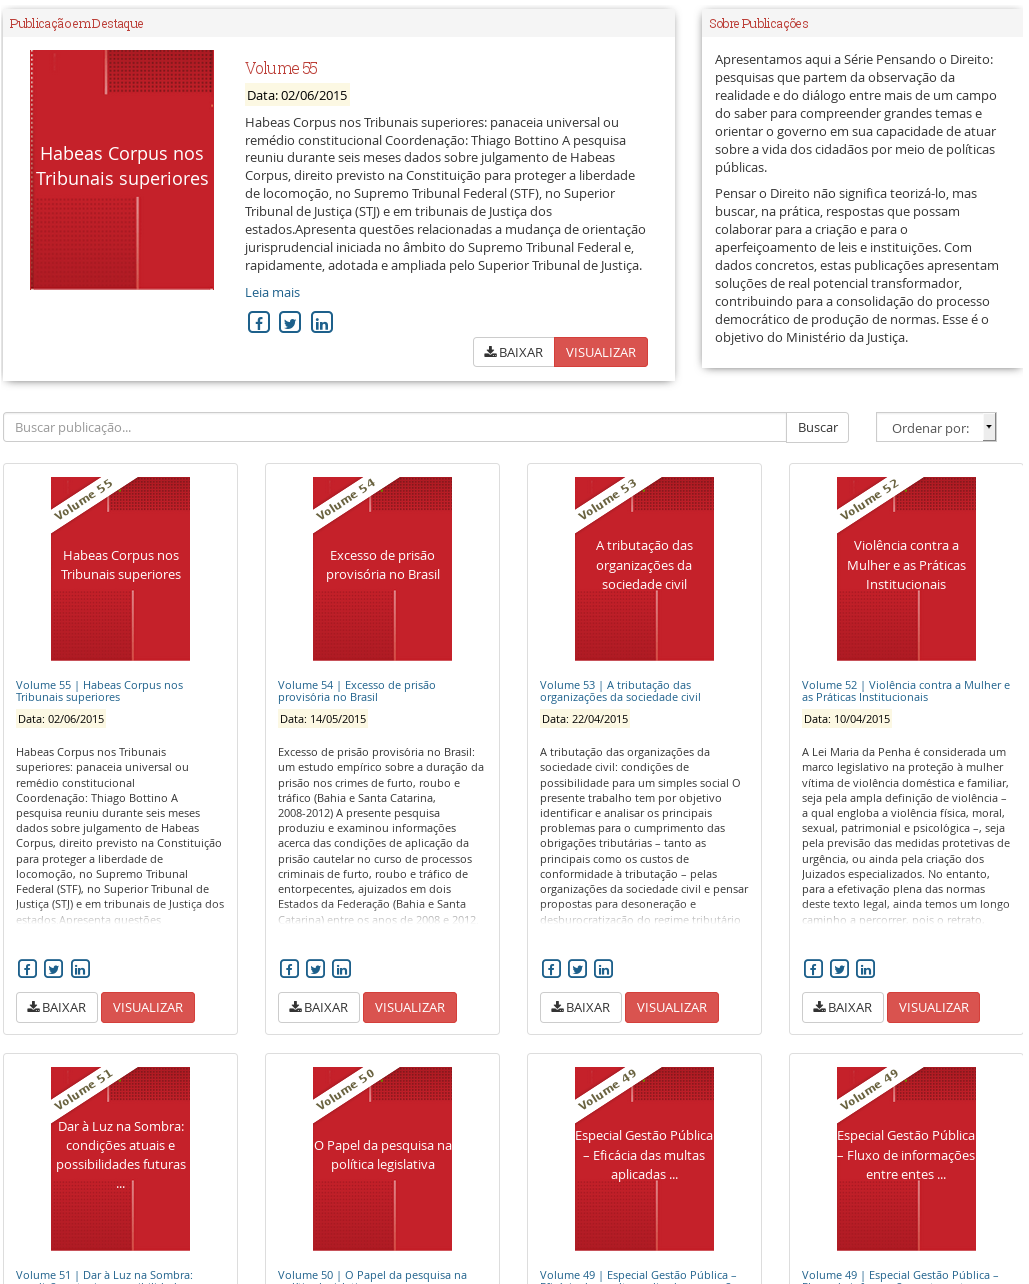
\includegraphics[scale=0.36]{./imagens/publicacoes-geral.png}%
	\end{center}%
	\caption{Página das Publicações\label{fig:publicacoes-geral}}%
	%\fonte{\url{http://participacao.mj.gov.br/}}%
\end{figure}%

Nesta área são apresentadas todas as publicações já disponibilizadas, com um destaque para a publicação mais recente - Figure \ref{fig:publicacoes-destaque}; e as demais em fileiras de 4 publicações, conforme pode ser observado na Figura \ref{fig:publicacoes-matriz}. As publicações nas fileiras serão apresentadas, por padrão, em ordem de publicação, da mais nova para a mais antiga.

\begin{figure}[htb]%
	\begin{center}
		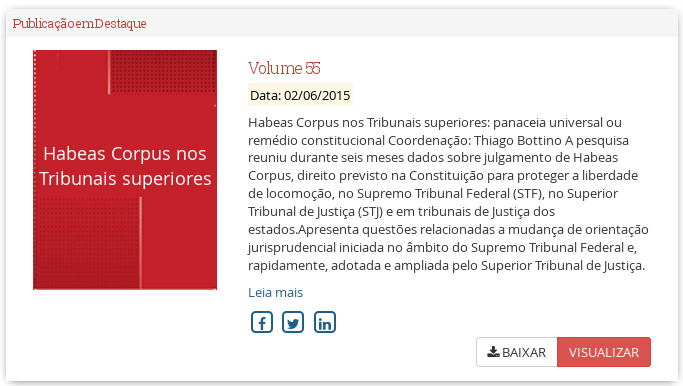
\includegraphics[scale=0.44]{./imagens/publicacoes-destaque.png}%
	\end{center}%
	\caption{Publicação em Destaque\label{fig:publicacoes-destaque}}%
	%\fonte{\url{http://participacao.mj.gov.br/}}%
\end{figure}%

Também há disponível a possibilidade de o usuário filtrar as publicações por meio de uma busca textual e mudar a regra de ordenação das publicações (por nome ou por número da publicação), conforme a Figura \ref{fig:publicacoes-busca}.

\begin{figure}[htb]%
	\begin{center}
		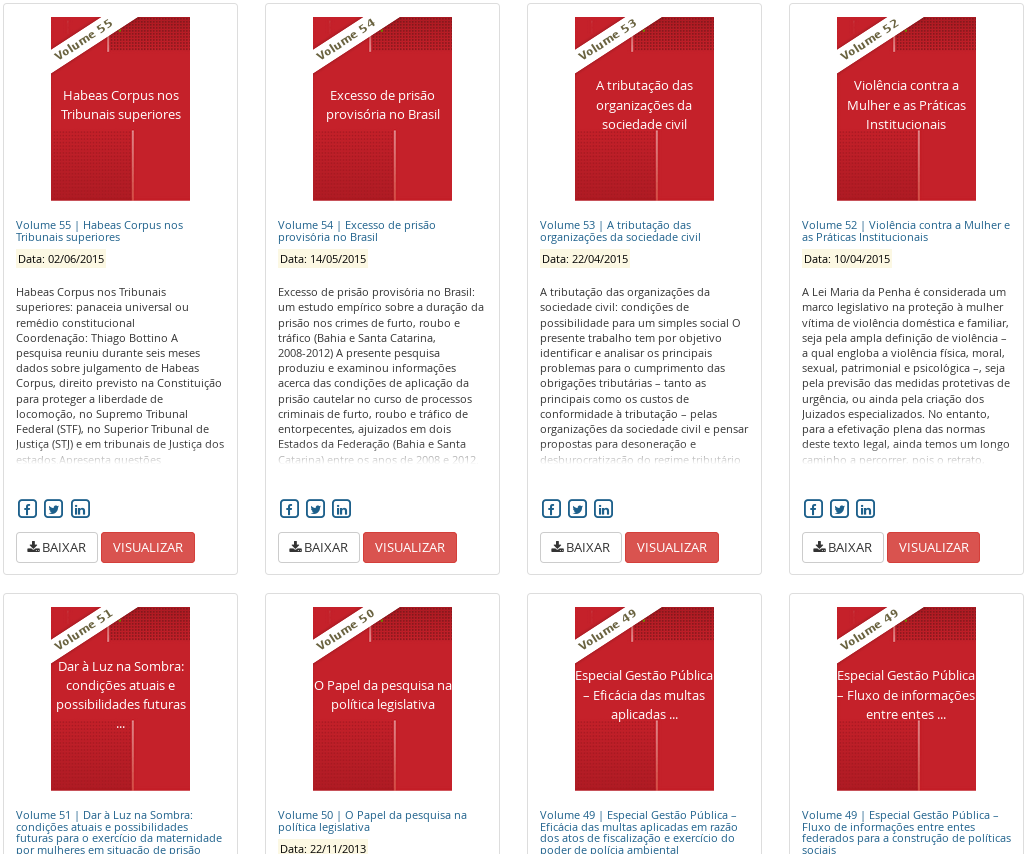
\includegraphics[scale=0.31]{./imagens/publicacoes-matriz.png}%
	\end{center}%
	\caption{Demais Publicações\label{fig:publicacoes-matriz}}%
	%\fonte{\url{http://participacao.mj.gov.br/}}%
\end{figure}%

Uma funcionalidade que não foi implementada, mas que sugere-se adicionar é o recurso que permita ao usuário escolher se deseja a ordenação das publicações apresentadas de forma ``crescente'' ou ``decrescente''. Uma boa solução seria utilizar a simbologia de setas para cima ou para baixo ao lado da caixa de seleção do tipo de ordenação que o usuário deseja. Esta sugestão foi registada como \textit{issue} de número 240\footnote{\textit{Issue} criada: \url{https://github.com/pensandoodireito/participacao-sitebase/issues/240}} no repositório de gestão do projeto\footnote{Repositório de gestão do projeto: \url{https://github.com/pensandoodireito/participacao-sitebase/issues}}.

Para melhorar a usabilidade e o desempenho para os usuários, inicialmente serão mostradas apenas as 9 publicações mais recentes - incluso o destaque; e ao final das mesmas é apresentado um botão "Mais Publicações" que irá carregar, dinâmicamente, mais uma fileira de 4 publicações a cada clique sobre o botão.

\begin{figure}[htb]%
	\begin{center}
		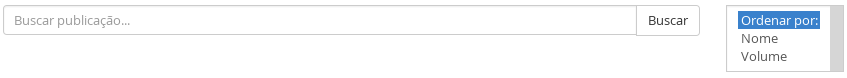
\includegraphics[scale=0.55]{./imagens/publicacoes-busca.png}%
	\end{center}%
	\caption{Busca das Publicações\label{fig:publicacoes-busca}}%
	%\fonte{\url{http://participacao.mj.gov.br/}}%
\end{figure}%

\subsubsection*{Página da Publicação}
Já na página de uma publicação específica, há um \textit{widget} ``outras publicações'', que traz outras publicações da série \ppod que versem sobre temáticas semelhantes ou que dialoguem com a publicação sendo visualizada. É preciso verificar o critério atual de escolhe destas publicações.

Nesta página há a possibilidade de o usuário visualizar o PDF da publicação na própria página, ler um resumo sobre a publicação, baixar o PDF da mesma, compartilhá-la nas redes sociais (Facebook, Twitter ou LinkedIn), ver os autores e autoras da Publicação e navegar para a publicação anterior ou para a próxima, caso elas existam.

Com relação ao compartilhamento nas redes sociais, é preciso verificar se as meta-informações da página estão configuradas de forma que o compartilhamento na rede social apresente uma imagem, além do texto, visto que a utilização de imagem aumenta o impacto da publicação nas redes sociais.

Sobre a visualização de autoras e autores, este recurso não foi completamente implementado pois não foi desenvolvido um campo específico para tal conteúdo.

A previsão inicial era de que os autores da publicação seriam apresentado junto a uma mini-biografia dos mesmos. Porém, não há na ferramenta um ``catálogo de autores'', que permita cadastrar previamente os autores e reutilizar esse cadastro. Dessa forma, a única solução mais direta seria a implementação de um campo extra (um \textit{array} num campo do tipo \textit{meta} do \gls{cpt}) que permita, a cada publicação, inserir o/a(s) autor(es)/autora(s)
e sua respectiva descrição. Esta abordagem não foi implementada por falta de tempo para o desenvolvimento da mesma e também pois ela demandaria recadastrar esta informação para todas as publicações já existentes na plataforma, mas recomenda-se que esta abordagem seja seguida. Após sua implementação no \textit{backend}, será necessário também implementá-la no front-end, criando a tela que apresentará este conteúdo, após o clique no link ``Ver autores'' que se apresenta logo acima dos botões de redes sociais. 

\subsubsection*{\textit{Widget} Publicações}
Foi desenvolvido um \gls{widget} para as publicações, que permite a inclusão de um \gls{sidebar} que faz referências a ``outras publicações'', conforme observado na figura \ref{fig:publicacoes-sidebar}.

A proposta deste \gls{widget} é ser utilizado na página que apresenta uma única publicação, trazendo outras publicações da série \ppod que versem sobre temáticas semelhantes ou que dialoguem com a publicação sendo visualizada.

É preciso verificar o critério atual de escolhe destas publicações.

\begin{figure}[htb]%
	\begin{center}
		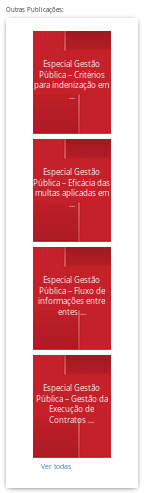
\includegraphics[scale=0.55]{./imagens/publicacoes-sidebar.png}%
	\end{center}%
	\caption{Sidebar das Publicações\label{fig:publicacoes-sidebar}}%
	%\fonte{\url{http://participacao.mj.gov.br/}}%
\end{figure}%


\subsection{Debates}
Os debates (consultas públicas) promovidos pela \gls{sal} são realizados por meio de ferramentas específicas, a depender do modelo de Debate Público - debate sobre texto ou debate sobre temas.

Estas ferramentas foram desenvolvidas e exploradas em outros produtos.

No que concerne ao Portal \ppod, em termos de codificação, a relação dos debates para com o Portal se dá de duas formas.

A primeira delas é a listagem dos debates, correntes e finalizados, no Portal, em página específica, e as chamadas para os debates na página principal.

Para esta primeira forma foi desenvolvido um novo \gls{cpt}, chamado ``\textit{arq\_debate\_post\_type}'', que servirá como arquivo histórico dos debates. Para cada novo debate que for ser iniciado, será preciso criar um novo conteúdo baseado neste \gls{cpt} com as informações do debate.

As informações referentes a este \gls{cpt} são:
\begin{description}
\item Título;
\item Descrição;
\item Imagem;
\item \textit{Status} - Estado do debate (Aberto ou Encerrado);
\item link - Endereço da página do debate;
\item período de - Quando se iniciou o debate;
\item período para - Quando o debate foi ou será finalizado;
\item assunto - Assunto do debate;
\item categoria - Categoria do debate;
\item fases - Quais fases ocorreram ou ocorrerão neste debate; e
\item resultados - Resultados do debate.
\end{description}

Os conteúdos referentes a este \gls{cpt} estarão disponíveis na página \url{http://pensando.mj.gov.br/debates}.

Futuramente este conteúdo pode ser evoluído para conter algumas estatísticas básicas de cada debate (como número de participantes), após encerrado, para apresentar estas informações na página de listagem dos debates.

\subsection{Proponha um Debate}
Um novo recurso que foi pensado/planejado é uma nova área para que a população possa participar do processo de formulação da Agenda dos Debates, permitindo a ela contribuir na priorização de temas a serem levados como Debates Públicos pela \gls{sal}.

Para este recurso será necessário criar um \gls{cpt} próprio, que se adeque ao modelo apresentado no produto desenvolvido pela consultora Mariana Lucchesi.

As ``telas'' para este novo fluxo de participação social já estão desenvolvidas estaticamente, mas é preciso criar os recursos do Wordpress para implementar as funcionalidades nelas presentes. As telas estão presentes no tema ``\textit{pensandoodireito-tema}'', e são as seguintes:
\begin{description}
\item \textit{page-comece-debate.php};
\item \textit{page-comece-novo-debate.php};
\item \textit{page-explore-e-vote.php};
\item \textit{page-proposta-comece-debate.php}; e
\item \textit{page-proposta-criada.php}.
\end{description}


\subsection{Programa de Intercâmbio}
Uma das ações da \gls{sal} é o Programa de Intercâmbio, voltado para estudantes de graduação e pós-graduação.

Este programa contava com um blog independente, desvinculado do projeto \ppod. Com o objetivo de fortalecer ambas iniciativas, o blog do projeto será integrado ao Pensando O Direito como um subsite.

Dessa forma, além de uma uniformização na linguagem visual dos sites, o blog do programa de intercâmbio também aparecerá no menu do Portal \ppod.

\subsection{Agenda}
Um novo recurso a ser implementado no portal é uma Agenda de Eventos, com as atividades da \gls{sal}.

Para esta agenda pode ser desenvolvido um novo \gls{cpt} ou pode-se buscar um plugin de eventos do Wordpress que ajude atenda as requisitos definidos, como por exemplo o \textit{events manager}\footnote{\textit{Events Manager}: \url{https://wordpress.org/plugins/events-manager/}}, sendo necessário apenas desenvolver o template para a agenda conforme a programação visual do Portal.

\subsection{Destaques}
Na página inicial há uma área de banner dedicada a destacar conteúdos específicos, de acordo com decisões da equipe de comunicação.

Para esta área foi desenvolvido um \gls{cpt} específico, chamado ``\textit{destaque\_post\_type}'', que permitirá que a equipe de comunicação possa criar, agendar, publicar e despublicar os destaques conforme a necessidade, sem que seja preciso interferência da equipe de desenvolvimento.

Este novo \gls{cpt} permite a adição de vídeo, imagem e texto, podendo o vídeo e a imagem serem acompanhadas de um textou ou não.

\subsection{Outras modificações}
Além do já exposto, algumas outras modificações foram realizadas.

As \textbf{Categorias} utilizadas para as \textbf{Notícias} foram padronizadas e reduzidas, facilitando a organização dos conteúdos. Caso se deseje adicionar informações mais detalhadas sobre uma notícia, o campo a ser utilizado deve ser o campo de \textbf{Tag}.

Uma das categorias criadas é a \textbf{Editais}, o que permitiu a criação de uma página dedicada aos Editais apenas filtrando as notícias pela categoria ``Editais''.

Outra mudança é que algumas páginas foram reeditadas e redesenhadas, como a página ``Conheça o Projeto''.

Por fim, diversas páginas de conteúdo estático - como a ``Parceiros'', agora são criadas automaticamente assim que o tema é ativado. Este código pode ser encontrado dentro do arquivo ``\textit{functions.php}'' do tema (\textit{pensandoodireito-tema} e \textit{participacao-tema}). Após criada, a página pode ser modificada no painel de administração do wordpress.

Futuras novas páginas estáticas sugere-se seguir o mesmo procedimento, pois assim evita-se esquecer de criar uma página que possui links e referências em diversas áreas do site.